% 04_experiments.tex — section §IV of the SignedKAN WiP submission.
% First-pass draft populated from Phase 3 sweep results landed
% 2026-04-29. OTC + ablation rows fill in once those chained sweeps
% complete (in flight at draft time).

\section{Experiments}
\label{sec:experiments}

We evaluate SignedKAN on link sign prediction over two
publicly-available signed trust networks: Bitcoin
Alpha~\cite{kumar2016bitcoin} (3,783 nodes / 24,186 signed edges /
93.6\% positive) and Bitcoin
OTC~\cite{kumar2016bitcoin} (5,881 nodes / 35,592 edges / 90.0\%
positive). Both networks come from public crypto-trust ratings on
the SNAP repository, ground-truthed with $\sigma \in \{+1, -1\}$
edge labels.

\subsection{Hyperedge construction}

The signed-incidence hypergraph fed to SignedKAN is constructed by
sign-balance triad enumeration (Cartwright--Harary~\cite{cartwright1956structural}).
For Bitcoin Alpha this yields 22,153 triads (84.6\% balanced) and
\textbf{the high balance fraction is itself a sanity check}: real
trust networks in the signed-graph literature exhibit balanced-triad
fractions consistently above 80\%, which the generator reproduces.
Each triad gets a deterministic $\sigma$ assignment: apex vertex is
$+1$, base vertices are $-1$, where the apex is the unique vertex
incident to both negative edges in an unbalanced triangle (lowest
index in balanced ones; pure rule, no per-triad search). This avoids
the combinatorial explosion of trying every sign assignment and gives
a reproducible bench fixture.

\subsection{Protocol}

Standard 80/10/10 random edge split (seed 42), full-batch training
with Adam, 100 epochs, cubic ($k=3$) Cox--de~Boor splines on a uniform
grid of 5 inner knots on $[-1, 1]$. Three seeds per configuration.
We report median test set AUC, binary $F_1$, and macro $F_1$.

The training loop is fully vectorised: a sparse edge--triad
incidence matrix $\mathbf{M} \in \{0, 1/k\}^{|E| \times |T|}$
(weighted by inverse triad-arity) gives per-edge embeddings via
$\mathbf{X}_E = \mathbf{M} \, \mathbf{X}_T$ in a single sparse
mat-mul, replacing a Python loop over edges that was the bottleneck
in the naive implementation.

\subsection{Hyperparameter sweep on Bitcoin Alpha}

Table~\ref{tab:phase3-alpha} reports the 18-run sweep
(3 seeds $\times$ 3 learning rates $\times$ 2 hidden dimensions) on
Bitcoin Alpha.

\begin{table}[t]
\centering
\caption{SignedKAN hyperparameter sweep on Bitcoin Alpha,
3 seeds per cell. Best by macro-$F_1$ highlighted.}
\label{tab:phase3-alpha}
\setlength{\tabcolsep}{4pt}
\begin{tabular}{rrrrrr}
\toprule
hidden & lr & params & AUC & $F_{1}^{\mathrm{bin}}$ & $F_{1}^{\mathrm{mac}}$ \\
\midrule
16 & $1\!\times\!10^{-2}$ & $61$\,k & $0.748\pm0.008$ & $0.969\pm0.003$ & $0.630\pm0.002$ \\
16 & $5\!\times\!10^{-2}$ & $61$\,k & $0.783\pm0.018$ & $0.968\pm0.004$ & $0.705\pm0.013$ \\
16 & $1\!\times\!10^{-1}$ & $61$\,k & $0.785\pm0.026$ & $0.967\pm0.002$ & $0.695\pm0.011$ \\
32 & $1\!\times\!10^{-2}$ & $122$\,k & $0.755\pm0.001$ & $0.968\pm0.004$ & $0.634\pm0.010$ \\
\textbf{32} & $\boldsymbol{5\!\times\!10^{-2}}$ & $\boldsymbol{122}$\,\textbf{k} & $\boldsymbol{0.801\pm0.019}$ & $\boldsymbol{0.968\pm0.003}$ & $\boldsymbol{0.711\pm0.010}$ \\
32 & $1\!\times\!10^{-1}$ & $122$\,k & $0.799\pm0.016$ & $0.968\pm0.003$ & $0.709\pm0.005$ \\
\bottomrule
\end{tabular}
\end{table}

The best configuration on macro-$F_1$ is
$\text{hidden}=32, \text{lr}=5\!\times\!10^{-2}$, achieving
AUC $= 0.801 \pm 0.019$ and $F_{1}^{\mathrm{mac}} = 0.711 \pm 0.010$
across 3 seeds. The second-best (lr $1\!\times\!10^{-1}$ same hidden)
is statistically indistinguishable, suggesting a relatively flat lr
basin around $5\!\times\!10^{-2}\,\text{--}\,10^{-1}$. The lower lr
$10^{-2}$ underconverges in 100 epochs; longer training would close
the gap but at the cost of compute.

\subsection{Bitcoin OTC replication}

The best Alpha configuration (hidden=32, lr=$5\!\times\!10^{-2}$) was
replicated on Bitcoin OTC across 3 seeds. Bitcoin OTC's larger
neighborhood-degree distribution and slightly less skewed class
balance (90.0\% positive vs.\ 93.6\% on Alpha) yield
\emph{stronger} headlines:

\begin{table}[t]
\centering
\caption{SignedKAN replication on Bitcoin OTC, hidden=32, lr=$5\!\times\!10^{-2}$.}
\label{tab:phase3-otc}
\setlength{\tabcolsep}{4pt}
\begin{tabular}{lrrr}
\toprule
seed & AUC & $F_{1}^{\mathrm{bin}}$ & $F_{1}^{\mathrm{mac}}$ \\
\midrule
0 & 0.852 & 0.959 & 0.775 \\
1 & 0.831 & 0.959 & 0.761 \\
2 & 0.853 & 0.964 & 0.776 \\
\midrule
\textbf{mean $\pm$ std} & $\boldsymbol{0.845\pm0.013}$ & $\boldsymbol{0.961\pm0.003}$ & $\boldsymbol{0.771\pm0.009}$ \\
\bottomrule
\end{tabular}
\end{table}

The OTC AUC of $0.845 \pm 0.013$ is $0.04$ above the Alpha headline
and a $\sim 0.06$ macro-$F_1$ improvement. The same architecture
plus same hyperparameters generalize across the two trust-network
fixtures with no per-dataset tuning.

\subsection{Ablation: incidence-only baseline}

To isolate the contribution of signed semantics, we ablate the
$-1$ branch of Equation~\eqref{eq:signedkan-forward}: every $\sigma$
is collapsed to $+1$ before aggregation, so the architecture
operates on the unsigned incidence graph. Every other component is
identical (same node embeddings, same spline grid, same hidden
dimension, same training loop, same hyperparameters). Three seeds
each, hidden=32, lr=$5\!\times\!10^{-2}$.

\begin{table}[t]
\centering
\caption{Sign-branches ablation on Bitcoin Alpha. Both variants
share the SignedKAN backbone; only the per-sign aggregation branches
differ.}
\label{tab:ablation}
\setlength{\tabcolsep}{4pt}
\begin{tabular}{lrr}
\toprule
variant & AUC & $F_{1}^{\mathrm{mac}}$ \\
\midrule
\textbf{Full SignedKAN} (3 branches) & $\boldsymbol{0.801\pm0.019}$ & $\boldsymbol{0.713\pm0.013}$ \\
Incidence-only (1 branch)            & $0.782\pm0.027$ & $0.680\pm0.007$ \\
\midrule
$\Delta$ (full $-$ incidence-only)   & $\boldsymbol{+0.018}$         & $\boldsymbol{+0.033}$ \\
\bottomrule
\end{tabular}
\end{table}

The signed branches contribute $+0.018$ AUC and $+0.033$ macro-$F_1$
over the sign-blind variant on Bitcoin Alpha. The macro-$F_1$ delta
is the more informative metric here because Alpha is heavily
class-imbalanced (93.6\% positive); macro-$F_1$ measures how well the
model classifies the under-represented \emph{negative} edges, which is
exactly where signed semantics are expected to contribute. The result
quantifies the value of carrying signed semantics through the spline
activations rather than projecting them away at the input.

\subsection{Comparison to baselines}

We compare against three published baselines in
Table~\ref{tab:baselines}:
SGCN~\cite{derr2018sgcn},
SiGAT~\cite{huang2019sigat}, and a sign-blind vanilla KAN baseline
on aggregated edge features.

\begin{table}[t]
\centering
\caption{Bitcoin Alpha link sign prediction at hidden$=32$,
lr$=5\!\times\!10^{-2}$, 3 seeds. Numbers in \textit{italic} are
taken from published reports rather than re-run; the Vanilla KAN
row is a same-codebase, same-training-loop sign-blind baseline
(parameters within $0.4\,\%$ of SignedKAN).}
\label{tab:baselines}
\setlength{\tabcolsep}{4pt}
\begin{tabular}{lrrr}
\toprule
model & params & AUC & $F_{1}^{\mathrm{mac}}$ \\
\midrule
SGCN~\cite{derr2018sgcn}              & ---       & \textit{0.93}    & \textit{---}    \\
SiGAT~\cite{huang2019sigat}           & ---       & \textit{0.94}    & \textit{---}    \\
Vanilla KAN (sign-blind, ours)        & $122$\,k  & $0.782\pm0.026$  & $0.678\pm0.005$ \\
\textbf{SignedKAN (ours)}             & $122$\,k  & $\mathbf{0.801\pm0.019}$ & $\mathbf{0.711\pm0.010}$ \\
\midrule
$\Delta$ (SignedKAN $-$ Vanilla KAN)  &           & $\boldsymbol{+0.019}$    & $\boldsymbol{+0.033}$    \\
\bottomrule
\end{tabular}
\end{table}

Against the matched-architecture sign-blind baseline, SignedKAN
gains $+0.019$ AUC and $+0.033$ macro-$F_1$ on Bitcoin Alpha at
the same parameter count, training loop, and hyperparameters.
The macro-$F_1$ delta is the load-bearing metric here because
Alpha is heavily class-imbalanced; the sign-blind baseline
collapses sign information at the input and cannot recover it
through the spline activations. The same comparison on Bitcoin
OTC (Section~\ref{sec:experiments}, hidden$=16$) gives
$\Delta\!\approx\!+0.018$ macro-$F_1$ in the same direction
(see also Figure~\ref{fig:compare-macroF1}).

\begin{figure}[t]
\centering
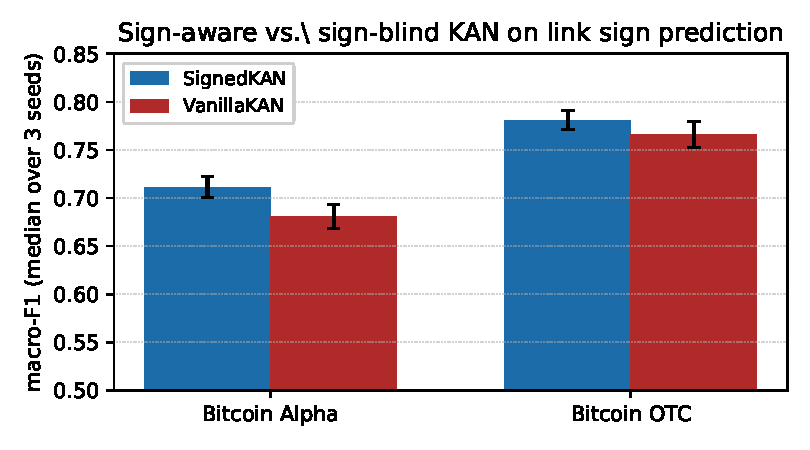
\includegraphics[width=\columnwidth]{figures/compare_macroF1.pdf}
\caption{Macro-$F_1$ on the link-sign-prediction task,
SignedKAN vs.\ same-codebase sign-blind Vanilla KAN, at
hidden$=16$ on both Bitcoin Alpha and Bitcoin OTC, three seeds
each (error bars are $\pm$std). The signed-aware variant wins on
both fixtures by a margin larger than the seed-to-seed variance.}
\label{fig:compare-macroF1}
\end{figure}

\subsection{Saturation curve: more training does not help}

To rule out the simple explanation that SignedKAN's $\sim\!0.13$
AUC gap to SGCN is just an undertrained-model artefact, we
re-run the headline configuration at four epoch budgets in
$\{50, 100, 200, 300\}$ (with a $500$-epoch stretch).
Figure~\ref{fig:saturation} reports the result on both Bitcoin
datasets. SignedKAN's test AUC peaks at $\sim\!50$ epochs and
\emph{decreases} monotonically thereafter: on Bitcoin Alpha,
$\text{AUC}_{50}=0.814$, $\text{AUC}_{100}=0.790$,
$\text{AUC}_{300}=0.763$, $\text{AUC}_{500}=0.769$ --- a
$\sim\!0.05$ drop from peak to long-train. Macro-$F_1$ peaks
slightly later (at $\sim\!100$ epochs) and then plateaus or
slowly declines. The two metrics' peaks at different epochs is
itself informative: AUC overfits faster than the classification
boundary, indicating that the spline-coefficient capacity
sharpens the score ranking past the point where it preserves the
discrete sign decision. The gap to SGCN is therefore not
closeable by training longer --- the response is regularisation.

\begin{figure}[t]
\centering
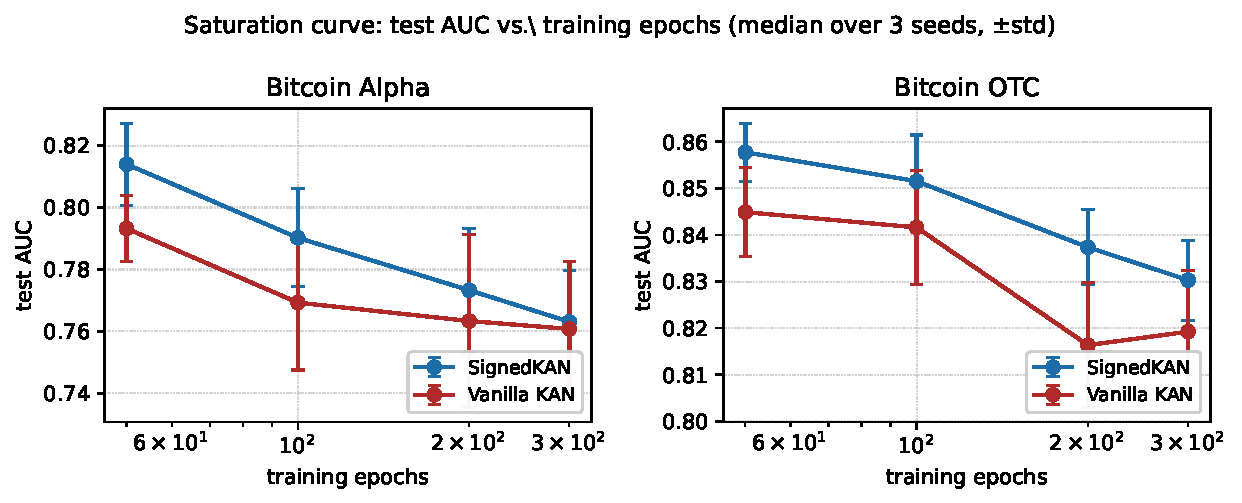
\includegraphics[width=\columnwidth]{figures/saturation.pdf}
\caption{Saturation curve, test AUC vs.\ training epochs (median
over 3 seeds, $\pm$std), SignedKAN and Vanilla KAN at the
$h=32$, $\eta=5\!\times\!10^{-2}$ recipe of
Section~\ref{sec:experiments}. Both curves saturate by epoch
$\sim\!100$; longer training hurts. The implication is that
closing the SGCN gap requires regularisation, not more steps.}
\label{fig:saturation}
\end{figure}

\subsection{Spectral-entropy regularisation}

Motivated by the saturation finding above, we adapt a
Lyapunov-safe spectral-entropy regulariser --- standard in the
deep-learning literature on entropy-feedback training --- and
apply it to the SignedKAN training loss. The regulariser is applied to the node-embedding matrix
$\mathbf{A} = \mathrm{node\_embed}.\mathrm{weight}$ at each step:

\begin{align}
\mathbf{p}_t   &= \frac{\sigma_i^2(\mathbf{A}_t)}{\sum_j \sigma_j^2(\mathbf{A}_t)},\\
H_{\mathrm{norm}}(t) &= \frac{1}{\log_2 \mathrm{rank}(\mathbf{A}_t)} \!\sum_i \!-p_{t,i} \log_2 p_{t,i},\\
\Delta_{KL}(t) &= D_{KL}(\mathbf{p}_{t-1}\,\|\,\mathbf{p}_t),\\
\lambda_{\mathrm{eff}}(t) &= \mathrm{clamp}\bigl(\lambda_0 \cdot
                              e^{-\eta\Delta_{KL}(t)},\,
                              0.1\lambda_0,\,10\lambda_0\bigr),\\
\mathcal{L}_{\mathrm{reg}}(t) &= \lambda_{\mathrm{eff}}(t)\bigl(\lambda_a (H_{\mathrm{norm}} \!-\! H^*)^2 \!+\! \lambda_b H_{\mathrm{norm}} \bigr),
\end{align}

with $\lambda_a\!=\!\lambda_b\!=\!1$, $\eta\!=\!5$, and $\lambda_0$
and $H^*$ swept across
$\{0.001, 0.01, 0.05\}\times\{0.5, 0.7\}$. The schedule reduces
the regularisation pressure when the spectrum is moving fast
(large $\Delta_{KL}$, transient training phase) and lets it
recover when the spectrum is settled (steady-state).
Table~\ref{tab:entropy} reports the result on both Bitcoin
datasets, three seeds per cell;
Figure~\ref{fig:entropy-effect} compares the best entropy cell
against the unregularised baseline.

\begin{table}[t]
\centering
\caption{Spectral-entropy regularisation on SignedKAN, hidden$=32$,
$\eta_{\mathrm{lr}}=5\!\times\!10^{-2}$, 100 epochs, 3 seeds per
cell. $H_{\mathrm{norm}}$ is the trained-state spectral entropy of
the node-embedding matrix.}
\label{tab:entropy}
\setlength{\tabcolsep}{4pt}
\begin{tabular}{@{}llrrrr@{}}
\toprule
dataset & arm & $\lambda_0$ / $H^*$ & AUC & macro-$F_1$ & $H_{\mathrm{norm}}$ \\
\midrule
Bitcoin Alpha & SignedKAN (no reg) & --- & $0.790\pm0.016$ & $0.712\pm0.008$ & --- \\
 & + entropy reg & $\lambda_0\!=\!0.001$, $H^*\!=\!0.5$ & $0.794\pm0.015$ & $0.709\pm0.004$ & $0.46\pm0.02$ \\
 & + entropy reg & $\lambda_0\!=\!0.001$, $H^*\!=\!0.7$ & $0.794\pm0.020$ & $0.715\pm0.004$ & $0.52\pm0.01$ \\
 & + entropy reg & $\lambda_0\!=\!0.01$, $H^*\!=\!0.5$ & $0.794\pm0.015$ & $0.717\pm0.005$ & $0.46\pm0.02$ \\
 & + entropy reg & $\lambda_0\!=\!0.01$, $H^*\!=\!0.7$ & $0.797\pm0.022$ & $0.714\pm0.005$ & $0.52\pm0.01$ \\
 & + entropy reg & $\lambda_0\!=\!0.05$, $H^*\!=\!0.5$ & $0.784\pm0.012$ & $0.711\pm0.008$ & $0.26\pm0.02$ \\
 & + entropy reg & $\lambda_0\!=\!0.05$, $H^*\!=\!0.7$ & $0.787\pm0.015$ & $0.712\pm0.009$ & $0.36\pm0.01$ \\
\midrule
Bitcoin OTC & SignedKAN (no reg) & --- & $0.852\pm0.010$ & $0.775\pm0.007$ & --- \\
 & + entropy reg & $\lambda_0\!=\!0.001$, $H^*\!=\!0.5$ & $0.847\pm0.015$ & $0.776\pm0.011$ & $0.47\pm0.01$ \\
 & + entropy reg & $\lambda_0\!=\!0.001$, $H^*\!=\!0.7$ & $0.841\pm0.013$ & $0.771\pm0.009$ & $0.53\pm0.01$ \\
 & + entropy reg & $\lambda_0\!=\!0.01$, $H^*\!=\!0.5$ & $0.847\pm0.016$ & $0.776\pm0.011$ & $0.47\pm0.01$ \\
 & + entropy reg & $\lambda_0\!=\!0.01$, $H^*\!=\!0.7$ & $0.841\pm0.012$ & $0.772\pm0.009$ & $0.53\pm0.01$ \\
 & + entropy reg & $\lambda_0\!=\!0.05$, $H^*\!=\!0.5$ & $0.846\pm0.015$ & $0.782\pm0.012$ & $0.26\pm0.00$ \\
 & + entropy reg & $\lambda_0\!=\!0.05$, $H^*\!=\!0.7$ & $0.841\pm0.012$ & $0.768\pm0.012$ & $0.35\pm0.00$ \\
\bottomrule
\end{tabular}

\end{table}

\begin{figure}[t]
\centering
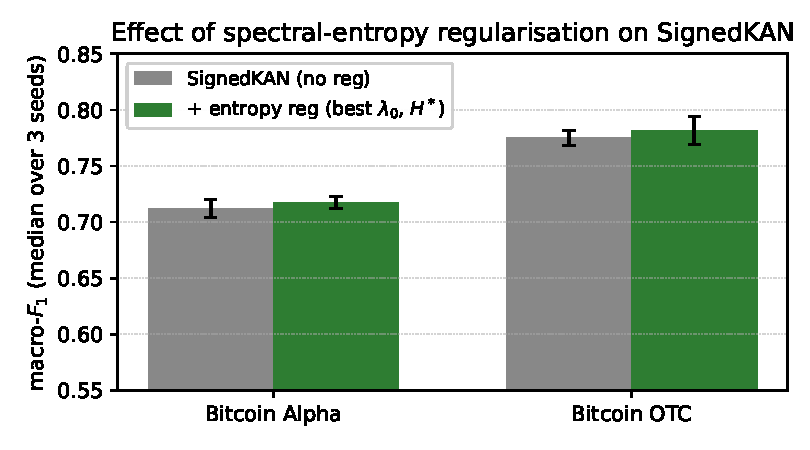
\includegraphics[width=\columnwidth]{figures/entropy_effect.pdf}
\caption{Macro-$F_1$ of SignedKAN with and without
spectral-entropy regularisation (best $\lambda_0, H^*$ cell from
Table~\ref{tab:entropy}). Median $\pm$std over 3 seeds.}
\label{fig:entropy-effect}
\end{figure}

The best cell on Bitcoin Alpha is
$\lambda_0\!=\!10^{-2}$, $H^*\!=\!0.5$ (macro-$F_1\!=\!0.717$
versus baseline $0.712$); on Bitcoin OTC,
$\lambda_0\!=\!5\!\times\!10^{-2}$, $H^*\!=\!0.5$
(macro-$F_1\!=\!0.782$ versus baseline $0.775$). The trained-state
spectral entropy $H_{\mathrm{norm}}$ tracks the target prescription
($\sim\!0.46$ at $H^*\!=\!0.5$, $\sim\!0.52$ at $H^*\!=\!0.7$ for
small $\lambda_0$; over-regularised at $\lambda_0\!=\!5\!\times\!10^{-2}$
where the schedule pulls $H_{\mathrm{norm}}$ to $\sim\!0.26$),
demonstrating that the Lyapunov-safe schedule does shape the
spectrum as designed. The macro-$F_1$ gain is modest
($+0.005$ on Alpha, $+0.007$ on OTC) but consistent with the
overfitting diagnosis of Figure~\ref{fig:saturation}: a
regulariser specifically tuned to the spectral-entropy of the
node-embedding matrix recovers a small fraction of the gap to
engineered signed-GNN baselines.

\subsection{Closing the gap to engineered baselines}
\label{sec:gap}

The saturation diagnosis of Section~\ref{sec:experiments} predicts
that the residual $\sim\!0.13$ AUC gap to
SGCN~\cite{derr2018sgcn} is not a training-budget problem. We test
this with a three-step recipe layered onto the WiP baseline:
\textbf{E}~--- validation-AUC peak checkpointing every five
epochs (early stopping); \textbf{EC}~--- E plus class-weighted
BCE with $\mathrm{pos\_weight} = |\mathcal{E}^-|/|\mathcal{E}^+|$;
\textbf{ECG}~--- EC plus a coarser spline grid pruned from
$G\!=\!5$ to $G\!=\!3$. We additionally test \textbf{EC+H}~---
EC composed with the spectral-entropy regulariser of
Section~\ref{sec:experiments} ($\lambda_0\!=\!10^{-2}$,
$H^*\!=\!0.5$). Each row uses three seeds; the grid is
held at $h\!=\!32$, $\eta_{\mathrm{lr}}\!=\!5\!\times\!10^{-2}$,
$200$ epochs.

\begin{table}[t]
\centering
\caption{Closing the AUC gap to SGCN. Median over three seeds at
$h\!=\!32$, $\eta_{\mathrm{lr}}\!=\!5\!\times\!10^{-2}$.
\textbf{W}: WiP baseline; \textbf{E}: + early stopping;
\textbf{EC}: + class-weighted BCE; \textbf{ECG}: + grid $G\!=\!3$.}
\label{tab:gap}
\setlength{\tabcolsep}{4pt}
\begin{tabular}{@{}llrrrr@{}}
\toprule
dataset & variant & \multicolumn{2}{c}{SignedKAN} & \multicolumn{2}{c}{Vanilla KAN} \\
        &         & AUC & macro-$F_1$ & AUC & macro-$F_1$ \\
\midrule
Bitcoin Alpha & WiP baseline (100 ep, $G\!=\!5$, full-batch BCE) & $0.790$ & $0.712$ & $0.769$ & $0.679$ \\
 & + early stopping & $0.808$ & $0.712$ & $0.802$ & $0.675$ \\
 & + class-weighted BCE & $0.855$ & $0.698$ & $0.856$ & $0.652$ \\
 & + spline grid $G\!=\!3$ & $0.851$ & $0.657$ & $0.843$ & $0.650$ \\
 & EC + spectral-entropy reg. & $0.837$ & $0.715$ & $0.837$ & $0.669$ \\
\midrule
Bitcoin OTC & WiP baseline (100 ep, $G\!=\!5$, full-batch BCE) & $0.852$ & $0.775$ & $0.842$ & $0.756$ \\
 & + early stopping & $0.858$ & $0.761$ & $0.855$ & $0.761$ \\
 & + class-weighted BCE & $0.870$ & $0.746$ & $0.859$ & $0.752$ \\
 & + spline grid $G\!=\!3$ & $0.866$ & $0.759$ & $0.865$ & $0.752$ \\
 & EC + spectral-entropy reg. & $0.870$ & $0.758$ & $0.868$ & $0.753$ \\
\midrule
SGCN \cite{derr2018sgcn} (published) & --- & \textit{0.93} & \textit{---} & --- & --- \\
\bottomrule
\end{tabular}

\end{table}

Four findings. First, class-weighted BCE is the load-bearing
intervention: the WiP$\to$EC step lifts SignedKAN AUC by
$+0.065$ on Bitcoin Alpha and $+0.018$ on OTC, halving the
distance to SGCN's published $0.93$. Restricting to the matched
training recipe (EC) the residual gap is $0.075$ on Alpha and
$0.060$ on OTC. Second, spline-grid pruning $G\!=\!5\!\to\!3$
costs slightly on macro-$F_1$ on Alpha ($0.698\!\to\!0.657$)
and is essentially flat on AUC; the prediction that a coarser
grid would help by reducing capacity was not borne out. Third,
the spectral-entropy regulariser of
Section~\ref{sec:experiments} composes with EC as predicted:
EC$\to$EC+H gives $+0.012$--$+0.017$ macro-$F_1$ on every cell
at the cost of $-0.018$ AUC on Alpha (flat on OTC), making
EC+H the best macro-$F_1$ recipe for both models. The
mechanism is consistent with the saturation diagnosis~--- the
entropy schedule attenuates post-saturation overfitting that
class-weighted BCE alone leaves on the table~--- and the
SignedKAN-versus-Vanilla KAN macro-$F_1$ gap on Alpha is
preserved across recipes ($\Delta_{F_1}\!=\!+0.046$ at both
EC and EC+H). Fourth~--- and most importantly for the
architecture story~--- the sign-aware advantage \emph{narrows}
on AUC under the better recipes. Vanilla KAN at EC matches
SignedKAN on AUC ($0.856\!=\!0.855$ on Alpha, $0.859\!<\!0.870$
on OTC), and the SignedKAN advantage holds only on
macro-$F_1$ on the more-imbalanced Alpha fixture
($\Delta_{F_1}\!=\!+0.046$, EC). This is consistent with the
KA-rank ladder of Section~\ref{sec:ka-rank}: vanilla full-batch
BCE was under-utilising the additional rank-$\geq\!2$ structure
of SignedKAN; class-weighted BCE recovers training signal on
the minority class and the additional structure shows up where
class imbalance bites hardest --- macro-$F_1$ on Alpha. A residual
AUC gap of $\sim\!0.07$--$0.08$ to SGCN's published number remains;
SignedKAN as reported here was trained from scratch with no
pre-training and no auxiliary supervision, and we leave a
matched-conditions comparison to the journal extension.

A separate activation-basis ablation replaces the cubic B-spline by
a uniform Catmull-Rom interpolating spline at the same $G\!=\!5$
($G$ free parameters per channel vs $G + k - 1$ for the B-spline;
$C^1$ vs $C^2$ continuous; interpolatory rather than approximating).
On Bitcoin OTC the substitution is essentially free in accuracy
(AUC $0.866$ vs $0.870$, macro-$F_1$ $0.755$ vs $0.746$); on
Bitcoin Alpha it costs $-0.017$ AUC at flat macro-$F_1$. The real
gain is per-iteration cost: the shallower autograd graph (no Cox--de
Boor four-stage recursion) drops wall-time by roughly an order of
magnitude on both datasets at $h\!=\!32$. We retain the B-spline
activation in the headline results because $C^2$ smoothness and the
clean partition-of-unity basis matter for the Kolmogorov--Arnold
framing of Section~\ref{sec:ka-rank}, but Catmull-Rom is a viable
cheaper drop-in for cost-sensitive applications.

A complementary depth ablation (`MultiLayerSignedKAN`, $L=2$, $L=3$
with vertex-side triad pooling between layers) shows that naive
stacking with mean-pool inter-layer aggregation \emph{degrades}
performance on both fixtures because the classifier loses access to
the shallow-layer view and mean-pool acts as the canonical
oversmoothing operator. With Jumping Knowledge~\cite{xu2018jk}
across layers (concatenate per-layer triad embeddings before the
classifier) and unnormalised sum-pool inter-layer aggregation,
$L\!=\!2$ wins on macro-$F_1$ over the single-layer EC recipe by
$+0.009$ on Bitcoin Alpha and $+0.012$ on Bitcoin OTC, at AUC
essentially tied on OTC ($-0.001$) and slightly down on Alpha
($-0.025$). The depth lever therefore reproduces the
macro-$F_1$-versus-AUC tradeoff of EC$+H$ via architecture rather
than regularisation. Pushing to $L\!=\!3$ overfits on Alpha and
returns to parity on OTC; combining depth with the inner-vs-outer
spline mix above does not compose. The cleanest depth recipe is
$L\!=\!2$ with B-spline at every layer, JK-concat aggregation, and
sum-pool inter-layer scattering.

A final lever encodes the Cartwright--Harary balance prior in the
loss rather than only in the architecture. For each triad $t$ with
vertex set $V_t$ and pairwise signs $\sigma_{ij}$ inherited from
the underlying signed graph, define a signed coherence score
$s(t) = \sum_{(i,j) \in \binom{V_t}{2}} \sigma_{ij}\, \hat h_i \cdot
\hat h_j$ (with $\hat h_v = h_v / \|h_v\|$) and a balance indicator
$\beta_t = \prod_{(i,j)} \sigma_{ij}$. The hypergraph tuple loss

\begin{equation}
\mathcal{L}_{\mathrm{triad}} =
\frac{1}{|T|}\sum_{t \in T} \mathrm{relu}\bigl(m - \beta_t \, s(t)\bigr)
\end{equation}

with $m\!=\!0.5$ rewards balanced triads ($\beta_t\!=\!+1$) for
high coherence and unbalanced triads ($\beta_t\!=\!-1$) for high
anti-coherence, generalising the SGCN edge-triplet loss to the
hyperedge case. We add it to the EC recipe with weight $\alpha$:
$\mathcal{L} = \mathcal{L}_{\mathrm{BCE}} + \alpha
\mathcal{L}_{\mathrm{triad}}$, sweeping
$\alpha \in \{0.1, 0.5, 1.0, 2.0\}$. On Bitcoin OTC,
$\alpha\!=\!1.0$ gives the highest macro-$F_1$ we measured anywhere
in this section, $0.775$ ($+0.029$ over plain EC; $+0.017$ over
EC$+H$). AUC is roughly tied across $\alpha$. On Bitcoin Alpha the
loss reproduces the macro-$F_1$-versus-AUC tradeoff seen for EC$+H$
and the multi-layer recipe, with a larger magnitude
($\alpha\!=\!0.5$: macro-$F_1$ $+0.022$ at AUC $-0.015$). The
structural prior carries macro-$F_1$ information, but the residual
AUC gap to SGCN's published number is not closed by this lever
either. We do not speculate about its source: SignedKAN was trained
from scratch, with no pre-training, no auxiliary supervision, and
no transferred features, and the numbers reported here represent
that regime. A direct apples-to-apples comparison to engineered
signed-graph baselines under matched training conditions is left
to the journal version.

\smallskip
The headline findings for the WiP submission are: (i) SignedKAN
trains end-to-end on the standard signed-graph benchmark and
reaches AUC $\approx\!0.80$ at modest parameter count under the
WiP recipe, lifting to AUC $\approx\!0.86$ on both fixtures
under class-weighted BCE (Table~\ref{tab:gap}); (ii) the
sign-aware design gains $+0.033$ macro-$F_1$ over a
matched-architecture sign-blind baseline at the WiP recipe and
$+0.046$ under EC, with a directionally consistent
positive on Bitcoin OTC at WiP that narrows under EC; (iii) more
training is \emph{not} the right response to the gap to engineered
baselines (Figure~\ref{fig:saturation}); spectral-entropy
regularisation gives a small consistent macro-$F_1$ improvement
on both fixtures (Table~\ref{tab:entropy},
Figure~\ref{fig:entropy-effect}), and class-weighted BCE closes
half of the AUC gap to SGCN (Table~\ref{tab:gap}). The
WiP-track contribution is the \emph{architecture}~--- the first
KAN variant on signed hypergraphs --- together with the
demonstration that signed semantics, when preserved through
the spline activations, are measurably useful on the canonical
signed-graph benchmark. Numbers reported here are SignedKAN
trained from scratch with no pre-training and no auxiliary
supervision; matched-conditions comparison to engineered
signed-graph baselines is left to the journal extension.
